% ---------------------------------------------------------------------------
% Hauptteil, Teil 1: Bisheriger Forschungsstand (Merkblatt 3.2)
% Demonstriert die Zitierweise im Fliesstext (Autor-Jahr, Seite nach Doppel-
% punkt) exakt nach den Beispielen des Merkblatts (S. 7).
% ---------------------------------------------------------------------------
\chapter{Forschungsstand}
\label{cha:forschungsstand}

In diesem Abschnitt wird der aktuelle Stand der Forschungsliteratur dargestellt. Zunächst werden die Faktoren erläutert, die die Integration von Geflüchteten in den Arbeitsmarkt beeinflussen. Anschließend werden veröffentlichte Forschungsergebnisse zum Effekt von Sprachkursen auf die Arbeitsmarktintegration von Geflüchteten vorgestellt. Darauf aufbauend werden die relevanten Befunde aus Forschungsberichten zu Sprache und Arbeitsmarktintegration dargestellt. Abschließend werden bestehende Forschungslücken aufgezeigt.

\section{Sprachkenntnisse und Arbeitsmarktintegration von Geflüchteten}
\label{cha:arbeitsmarktintegration}

Im Allgemeinen besteht ein positiver Zusammenhang zwischen dem Spracherwerb der Zugewanderten in der Aufnahmelandessprache und ihren Einkommens- und Beschäftigungsaussichten \parencites{doi:10.1086/298374}{10.1111/1468-0297.t01-1-00151}. Der Spracherwerb hat deshalb für Zugewanderte einen besonderen Stellenwert auf dem Arbeitsmarkt.

Der Zusammenhang zwischen Sprachkompetenz und Arbeitsmarkterfolg gilt auch für Geflüchtete. Es liegen Belege dafür vor, dass Sprachkompetenz in einem positiven Zusammenhang mit der Beschäftigungs- und beruflichen Situation von Geflüchteten steht. Geflüchtete sind auf den Arbeitsmärkten der europäischen Länder benachteiligt, allerdings bestehen Unterschiede zwischen den verschiedenen Ländern \parencites{dumont2016refugees}{doi:10.1111/j.1747-7379.2010.00810.x}.

Der Spracherwerb ist nicht für alle Berufsgruppen von derselben Bedeutung. Je nach beruflicher Position können von Geflüchteten unterschiedliche Sprachkenntnisse verlangt werden. Der Spracherwerb bzw. das Sprachniveau kann im Kontext des Arbeitsmarktes einen unterschiedlichen Stellenwert haben \parencite{chiswick2010occupational}.

Auch für Flüchtlinge in Deutschland hat der Spracherwerb im Aufnahmeland im Hinblick auf die Integration in den Arbeitsmarkt an Bedeutung gewonnen. Bessere Sprachkenntnisse stehen auch bei Flüchtlingen in Deutschland in Zusammenhang mit der Beschäftigung \parencite{kosyakova2017large}. Darüber hinaus wurde gemäß der zweiten Erhebungswelle der IAB-BAMF-SOEP-Umfrage festgestellt, dass sowohl die Sprachkenntnisse als auch die Beschäftigungsquoten von Geflüchteten in Deutschland im Laufe der Zeit gestiegen sind \parencite{brucker2019gefluchtete}.

Der Spracherwerb ist kein statischer Vorgang, sondern entwickelt sich über einen bestimmten Zeitraum und einen bestimmten Prozess hinweg. Neben individuellen Faktoren kann auch ein strukturierter Lernprozess den Spracherwerb von Zugewanderten fördern. Dies zeigt, dass der Spracherwerb nicht nur durch den individuellen Lernprozess, sondern auch durch strukturierte Angebote wie beispielsweise Sprachkurse gefördert werden kann \parencite{Kosyakova04042022}.

\section{Empirische Evidenz zur Wirkung von Sprachkursen}
\label{cha:empirische}

Die bisherige Forschungsliteratur zeigte, dass die Teilnahme an Sprachkursen und der Erwerb der deutschen Sprache zu den wichtigsten Faktoren gehören, die den Erfolg auf dem Arbeitsmarkt fördern \parencites{brucker2019language}{lang2022employment}{marbach2025does}. Der aktuelle Stand der Forschung zeigt, dass Sprachkurse die Integration in den Arbeitsmarkt fördern. Aus den aktuellen Forschungsergebnissen geht hervor, dass Sprachkurse nicht nur das Erlernen der Sprache des Aufnahmelandes erleichtern, sondern auch dazu beitragen, dass Geflüchtete spezifische arbeitsmarktrelevante Kenntnisse und Fähigkeiten erwerben \parencite{iza:izadps:dp16091}. Sprachtraining hat somit, wie in aktuellen Studien dargelegt, einen positiven Einfluss auf die Integration in den Arbeitsmarkt. Die bisherige Forschungsliteratur zeigt, dass Sprachkurse dafür sorgen, dass Geflüchtete bessere Deutschkenntnisse erwerben, wodurch sich ihre Chancen auf eine Teilhabe am Arbeitsmarkt verbessern \parencites{lang2022employment}{marbach2025does}.

Der Forschungsstand unterscheidet, welche Deutschkurse im Hinblick auf den Arbeitsmarkt am erfolgreichsten sind. \textcite{marbach2025does} haben analysiert, dass nicht alle Sprachenkurse gleichermaßen effektiv sind. Es hat sich gezeigt, dass kurzfristige Sprachenkurse, wie beispielsweise Ad-hoc-Kurse, keinen signifikanten Einfluss auf die Beschäftigung haben \parencite{marbach2025does}. Im Vergleich zu kurzfristig angelegten Kursen haben sich langfristig angelegte und umfassendere Kurse im Hinblick auf die Arbeitsmarktintegration von Geflüchteten als effizienter erwiesen \parencite{marbach2025does}. 

\textcite{lang2022employment} analysierte die Auswirkungen von Sprachkursen auf beschäftigungslose Zugewanderte. Sie stellte fest, dass Personen, die an berufsbezogenen Sprachkursen des BAMF teilnahmen, höhere Beschäftigungsquoten aufwiesen \parencite{lang2022employment}. Berufsbezogene Kurse zielen inhaltlich nicht nur auf den Erwerb der deutschen Sprache ab, sondern sind eine Kursart, die auch die Förderung arbeitsmarktspezifischer Sprachkompetenzen wie berufliche Kommunikation und Deutsch am Arbeitsplatz zum Ziel hat \parencite{lang2022employment}. Berufssprachkurse verbessern nicht nur die Deutschkenntnisse der Teilnehmenden, sondern tragen auch zur Erweiterung ihrer arbeitsmarktrelevanten Kenntnisse bei und wirken sich somit positiv auf ihre Beteiligung am deutschen Arbeitsmarkt aus. Dieses Ergebnis ist insbesondere in der Anfangsphase stärker ausgeprägt und bei Frauen im Vergleich zu Männern deutlicher zu erkennen \parencite{lang2022employment}. Zusammenfassend lässt sich festhalten, dass nicht jeder Sprachkurs die Integration von Geflüchteten in den Arbeitsmarkt in gleichem Maße beeinflusst; insbesondere Sprachkurse, die arbeitsmarktrelevante Kompetenzen fördern, haben sich positiv auf Beschäftigung und Einkommen ausgewirkt \parencite{lang2022employment}

\section{Aufenthaltsstatus und Arbeitsmarktintegration}
\label{cha:aufenthaltsstatus}

Im Vergleich zu anderen Zugewanderten sind Geflüchtete beim Spracherwerb und bei der Beschäftigungssuche mit gewissen Nachteilen konfrontiert \parencites{10.3389/fpos.2022.977764}{10.1093/epolic/eix008}. Einer der zentralen Faktoren für den Erfolg von Geflüchteten auf dem Arbeitsmarkt ist das Zielsprachenerlernen \parencite{Kosyakova04042022}. Aus diesem Grund bieten viele Aufnahmeländer, wie beispielsweise Deutschland, Sprach- und Integrationskurse für Geflüchtete an \parencite{kristen2021destination}.

\textcite{Kanas:2023} haben den kausalen Zusammenhang zwischen lokalen Sprachkursen in Deutschland und den Beschäftigungsaussichten von Geflüchteten untersucht. Die Analyse ergab, dass ein hohes Angebot an Sprachkursen in dem Landkreis, in den Geflüchtete zugewiesen werden, ihre Beschäftigungsaussichten verbessert. Der Zusammenhang zwischen dem Angebot an lokalen Sprachkursen und der Beschäftigung wurde zudem anhand von Mechanismen wie dem Abschluss eines Sprachkurses, der Häufigkeit des Kontakts zu Deutschen und der Sprachkompetenz untersucht.

Der Zusammenhang zwischen dem Aufenthaltsstatus von Geflüchteten und dem Arbeitsmarkt wurde in der Forschungsliteratur intensiv untersucht. Bisherige Untersuchungen zeigen, dass der ungewisse Aufenthaltsstatus von Geflüchteten und die lange Dauer des Asylverfahrens zu Verzögerungen bei der Integration der Geflüchteten in den Arbeitsmarkt führten \parencites{article}{doi:10.1126/sciadv.1600432}.

Unabhängig vom Ergebnis des Aufenthaltsstatus haben bisherige Untersuchungen gezeigt, dass eine schnelle Klärung des Aufenthaltsstatus dazu beitragen kann, dass Geflüchtete schneller mit einem Sprachkurs beginnen und eine Beschäftigung aufnehmen können \parencite{kosyakova2020role}. In diesem Zusammenhang wurde darauf hingewiesen, dass nicht nur der Aufenthaltsstatus, sondern auch ein schneller Ablauf des Asylverfahrens eine wichtige Rolle spielt. 

\textcite{10.1257/aer.89.2.186} erläutern, dass Migrant:innen entsprechend ihren eigenen Zielen in Humankapital investieren und dabei eine Kosten-Nutzen-Abwägung entsprechend ihren Zielen vornehmen. Dem zentralen Ergebnis zufolge führt ein sicherer Aufenthaltsstatus bei Migrant:innen dazu, dass sie einen höheren Nutzen aus ihren zielgerichteten Investitionen erwarten. Das heißt, aus der Perspektive der Bleibeperspektive kann ein sicherer Aufenthaltsstatus dazu führen, dass Migrant:innen einen größeren Nutzen aus den getätigten Investitionen erwarten \parencite{10.1257/aer.89.2.186}.

\textcite{repec:iab:iabdpa:202031} wenden diesen Gedanken in Form eines Choice-Experiments auf Deutschland an. Zu den zentralen Schlussfolgerungen gehört, dass die Gewissheit über die Zukunft der Geflüchteten in Deutschland sie dazu motivieren könnte, in Humankapital wie Sprache und Bildung zu investieren. Außerdem wird darauf hingewiesen, dass ein sicherer Aufenthaltsstatus dazu motiviert, in Humankapital wie Sprache und Ausbildung zu investieren \parencite{repec:iab:iabdpa:202031}.

Neben dem rechtlichen Aufenthaltsstatus kann auch die subjektive Bleibeabsicht der Zugewanderten im Zielland die Integration beeinflussen. \textcite{doi:10.1177/09500170261425857} unterteilten die Geflüchteten in drei verschiedene Gruppen: diejenigen, die dauerhaft bleiben möchten, diejenigen, die vorübergehend bleiben möchten, und diejenigen, deren Bleibeabsicht unklar ist. Das wichtigste Ergebnis ist die Beobachtung, dass Geflüchtete, die eine vorübergehende Bleibeperspektive im Aufnahmeland haben, im Vergleich zu denen, die dauerhaft bleiben möchten, geringere Sprachkenntnisse aufweisen. Außerdem wird eine unklare Bleibeperspektive im Aufnahmeland als nachteilig für den Spracherwerb der Geflüchteten erklärt \parencite{doi:10.1177/09500170261425857}.

Insgesamt zeigte die bisherige Forschung, dass Statusunsicherheit und längere Asylverfahren den Integrationsprozess von Flüchtlingen verlangsamen können \parencites{article}{doi:10.1126/sciadv.1600432}. Zudem wurde beobachtet, dass Flüchtlinge, die über einen sicheren Aufenthaltsstatus verfügen, durch Investitionen in Humankapital – wie Sprache und Bildung – größere Gewinne erzielen können \parencite{10.1257/aer.89.2.186}. Schließlich steht auch die subjektive Bleibeabsicht in Zusammenhang mit der Integration in den Arbeitsmarkt \parencite{doi:10.1177/09500170261425857}.



\section{Der deutsche Kontext}
\label{cha:deutsche_kontext}


\subsection{Das deutsche Integrations- und Sprachkurssystem}
\label{sec:deu-integ}

Ein Großteil der Fluchtbewegung der letzten Jahren fand zwischen 2015 und 2019 statt, und im Jahr 2016 stellten 722.370 Personen in Deutschland einen Asylantrag \parencite[13]{BAMF2020}. Deutschland ist daher in den letzten Jahren im Zusammenhang mit der Fluchtbewegung zu einem Zielland geworden \parencite{https://doi.org/10.1111/1467-9361.00008}. Dieser Anstieg der Fluchtbewegung seit 2015 hat auch zu politischen Veränderungen hinsichtlich der integrationspolitischen Maßnahmen in Deutschland geführt. 

Die Inhalte der vom BAMF durchgeführten Integrationskurse umfassten sowohl die Zielsprache als auch kulturelle Komponenten. Integrationskurse in Deutschland werden vom Staat organisiert und gelten als wichtiges Instrument für die Integration von Geflüchteten in Deutschland. Die Hauptaufgabe der Integrationskurse besteht darin, Deutschkurse für Migranten in Deutschland, vor allem für Geflüchtete, anzubieten. Das Ziel der Sprachkurse ist das Sprachniveau GER B1 \parencite{council2001common}. Neben der sprachlichen Förderung zielen sie darauf ab, grundlegende Kenntnisse über das Rechtssystem, die Geschichte und die Kultur Deutschlands zu vermitteln \parencite{Rother_2014}. Der allgemeine Kurs umfasst 600 Stunden Sprachunterricht, während der Orientierungskurs aus 100 Stunden besteht. Das übergeordnete Ziel besteht darin, die soziale und wirtschaftliche Integration von Geflüchteten in Deutschland zu fördern \parencite{Rother_2014}.

Personen, die in Deutschland einen Asylantrag gestellt haben, erhalten Berechtigungsscheine bzw. eine Teilnahmeberechtigung für die Teilnahme an Integrationskursen. Anfangs wurde das Teilnahmerecht nur Personen mit anerkanntem Asylantrag gewährt, jedoch wurde das Teilnahmerecht im Jahr 2015 erweitert \parencite{kosyakova2020role}. Auch Personen, bei denen die Wahrscheinlichkeit einer Anerkennung ihres Asylantrags hoch ist, sowie Personen, deren Asylantrag noch geprüft wird, erhielten das Recht zur Teilnahme an den Kursen. Auch in Ausnahmefällen erhielten Asylbewerber mit Duldungsstatus das Recht auf Teilnahme \parencite{kosyakova2020role}.

Zwischen 2014 und 2016 stieg die Zahl der Integrationskurse auf das Doppelte. Die Zahl der im Jahr 2016 begonnenen Integrationskurse erreichte 20.000 \parencite{grote2018changing}. Neben den vom Staat organisierten Kursen gab es weitere Programme, die von Bundesländern, Kommunen, zivilgesellschaftlichen Organisationen und Hilfsorganisationen angeboten wurden \parencites{kosyakova2020role}{brucker2020has}. Das Besondere an den Integrationskursen ist, dass sie neben dem Sprachunterricht eine umfassendere Integrationsförderung bieten. Obwohl die Zahl der Sprachkurse deutschlandweit gestiegen ist, blieb die Teilnehmerzahl hinter den Erwartungen zurück. Zwischen 2013 und 2016 nahm nur ein Drittel der Personen, die in Deutschland einen Asylantrag gestellt hatten, an einem Integrationskurs teil. Im Jahr 2017 stieg dieser Anteil jedoch an, sodass 55 Prozent der Betroffenen an einem Integrationskurs teilnahmen.


\subsection{Regionale Variation des Kursangebots}
\label{sec:erg-angebot}

Die Entwicklung der Integrationskurse in Deutschland zwischen den Jahren 2015 und 2016 ist in \ref{fig:kursangebot}  dargestellt. Panel A veranschaulicht die prozentuale Entwicklung der Integrationskurse auf Landkreisebene. Panel B zeigt die prozentuale Entwicklung der Erteilung von Teilnahmeberechtigungen für Sprachkurse für Geflüchtete zwischen 2015 und 2016. Abbildung~\ref{fig:kursangebot} ermöglicht einen Vergleich zwischen der Entwicklung der Integrationskurse und der Entwicklung der Berechtigungsbescheinigungen für Sprachkurse im Zeitraum von 2015 bis 2016.


\begin{figure}[htbp]
	\centering
	% Der Vektor-Master liegt als figures/fig01_both_panels.svg vor. XeLaTeX kann
	% SVG nicht direkt einbinden (dafuer waeren das svg-Paket, Inkscape und
	% --shell-escape noetig, was build.sh bewusst nicht verwendet); eingebunden
	% wird daher die 300-dpi-PNG-Fassung derselben Grafik.
	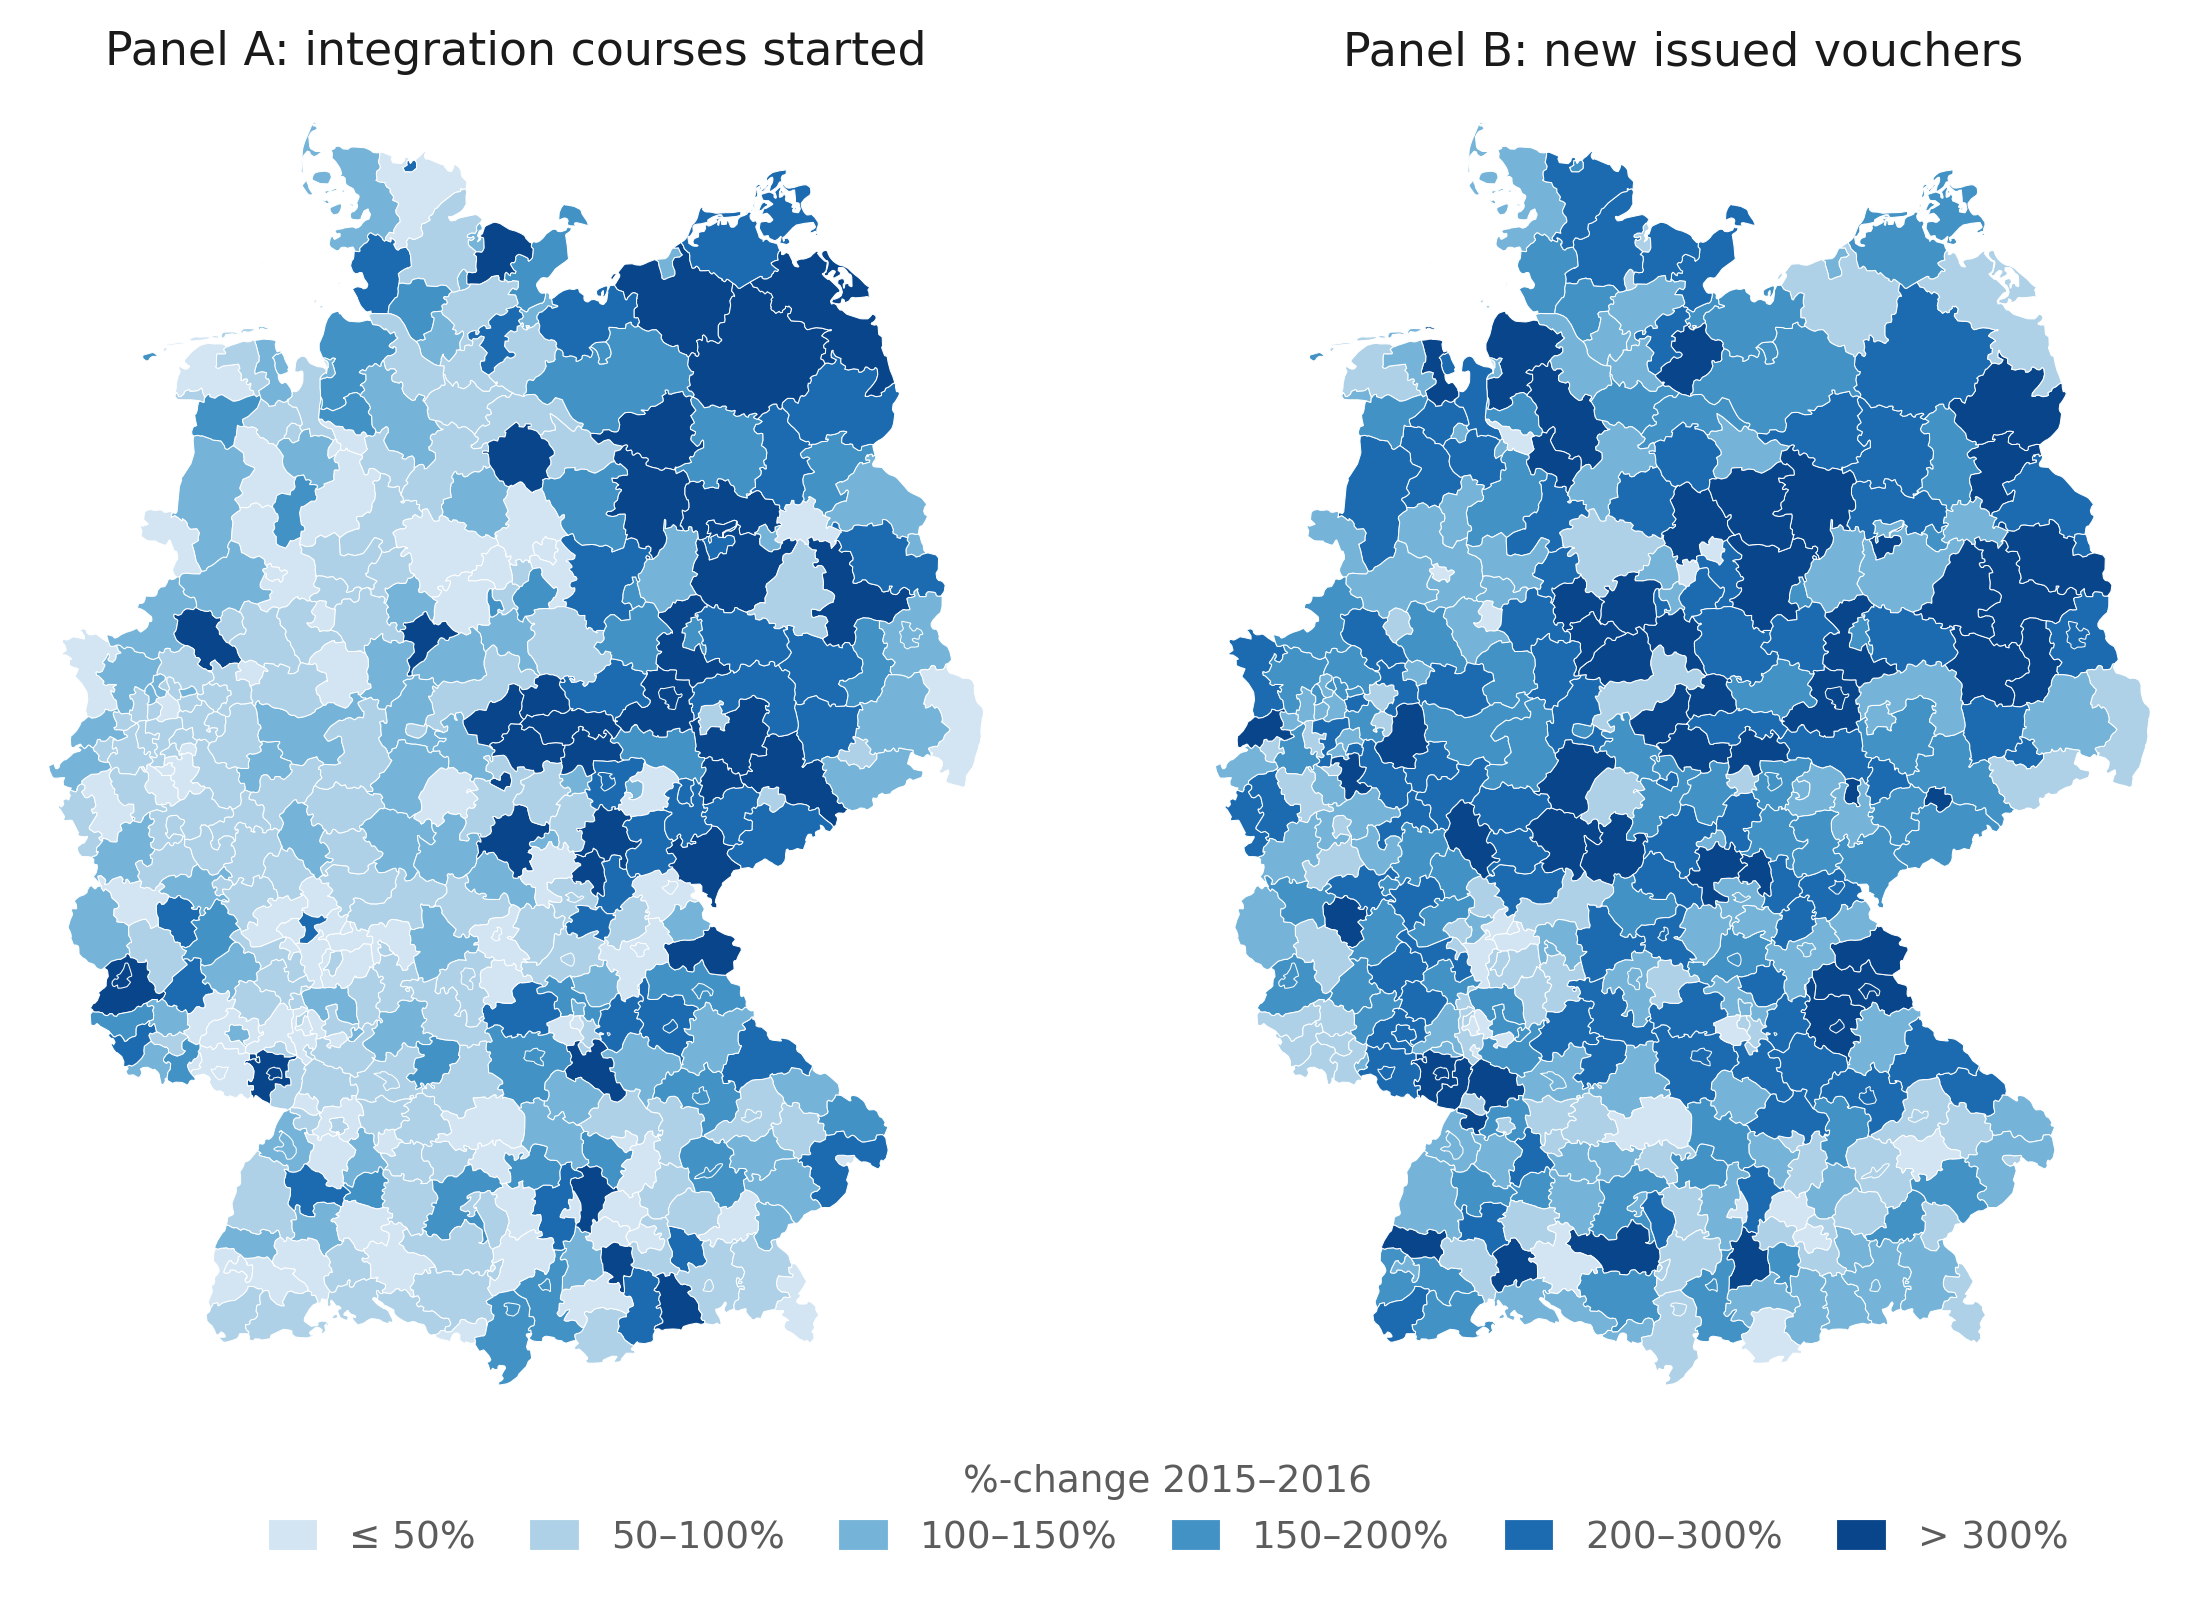
\includegraphics[width=\textwidth]{figures/fig01_both_panels.png}
	\caption[Ver\"anderung des Angebots an Integrationskursen 2015--2016 nach
	Kreisen]{Ver\"anderung des Angebots an Integrationskursen zwischen 2015 und
		2016 nach Kreisen. Panel~A: begonnene Integrationskurse; Panel~B: neu
		ausgestellte Berechtigungsscheine. Eigene Darstellung auf Basis der
		BAMF-Kursstatistik; Kreisgrenzen nach VG2500 (BKG). Entspricht Abbildung~1
		in \textcite{Kanas:2023}.}
	\label{fig:kursangebot}
\end{figure}

Sowohl Panel A als auch Panel B zeigen, dass zwischen den Kreisen deutliche Unterschiede zu beobachten sind. In einigen Kreisen steigt der Anteil der Integrationskurse, während der Anstieg in anderen Kreisen geringer ausfällt. Ähnliches gilt auch für die Berechtigungsbescheinigungen, die zum Kursbesuch für Geflüchtete ausgestellt werden. Während der Anstieg bei den ausgegebenen Berechtigungsbescheinigungen in einigen Regionen gering ist, ist er in anderen Regionen sehr deutlich. Aus diesem Grund ist die Entwicklung der Integrationskurse in Deutschland nicht in gleichem Maße vorangeschritten.

Die reproduzierte \ref{fig:kursangebot} zeigt uns, dass die Entwicklung der Integrationskurse in einem Kreis und die Zunahme der ausgestellten Berechtigungsnachweise nicht unbedingt im gleichen Maße verlaufen. Während die Angebot an Integrationskursen in einem Kreis zunimmt, kann es sein, dass bei ausgegebenen Berechtigungsnachweisen kein sichtbarer Anstieg zu beobachten ist. \ref{fig:kursangebot} zeigt auch, dass das genaue Gegenteil der Fall sein kann. Damit wird veranschaulicht, dass regionale Unterschiede zwischen Angebot und Nachfrage bei Integrationskursen auftreten können.

Beim Vergleich verschiedener Kreise in Deutschland lassen sich auffällige Unterschiede feststellen. Sowohl bei den Integrationskursen als auch bei der Entwicklung der Berechtigungsnachweise gibt es Unterschiede auf Kreisebene. Dies lässt sich so interpretieren, dass es auf Kreisebene zu regionalen Unterschieden beim Zugang zu Integrationskursen führen kann.

\textcite{Kanas:2023} zeigen, dass sich die Zahl der Berechtigungsnachweise in 165 Kreisen um mehr als das Doppelte erhöht hat. Die Zahl der Integrationskurse hat sich jedoch im Vergleich zum Vorjahr in weniger als der Hälfte der 165 Kreise verdoppelt. Dies lässt sich damit erklären, dass die Nachfrage nach Integrationskursen in einem Kreis nicht im gleichen Maße zugenommen hat wie die Entwicklung der Integrationskurse.

Insgesamt bestehen regionale Unterschiede hinsichtlich der Entwicklung der Integrationskurse und der an Geflüchtete ausgestellten Teilnahmebescheinigungen. Beispielsweise ist nicht zu beobachten, dass das Angebot an Integrationskursen in einem Kreis im gleichen Maße zunimmt mit der Anzahl der ausgestellten Teilnahmebescheinigungen.

\subsection{Arbeitsmarktzugang von Geflüchteten}
\label{sec:arb-zugang}

Der Zugang von Geflüchteten zum Arbeitsmarkt wird durch rechtliche Verfahren zentral geregelt. Die Arbeitserlaubnisse für Geflüchtete unterscheiden sich von anderen Migranten und können teilweise restriktiv sein. Das Herkunftsland und die aufenthaltsrechtliche Situation der Geflüchteten spielen in diesem Zusammenhang eine wesentliche Rolle \parencite{kosyakova2020role}.

Während Personen, deren Asylantrag noch nicht abgeschlossen ist, in den ersten drei Monaten keine Arbeitserlaubnis erhalten, können diese Personen danach unter bestimmten rechtlichen Voraussetzungen eine Arbeitserlaubnis erhalten. Personen, deren Asylverfahren noch nicht abgeschlossen ist, haben aus diesem Grund nur eingeschränkten Zugang zum Arbeitsmarkt \parencite{kosyakova2020role} .

Personen, deren Asylantrag anerkannt wurde, verfügen über unterschiedliche Schutzstatus. Diese Schutzstatus lassen sich wie folgt auflisten: Asylberechtigte, Personen mit subsidiärem Schutzstatus und Personen mit nationalem Abschiebungsverbot. Für Personen mit diesen Schutzstatus gelten keine Einschränkungen hinsichtlich der Beschäftigung \parencite{muller2016unterstutzungsmassnahmen}.

Der Arbeitsmarktzugang von Personen mit Duldungsstatus ist in Deutschland ebenfalls eingeschränkt; eine Arbeitserlaubnis wird nur unter bestimmten gesetzlichen Voraussetzungen erteilt \parencites{kosyakova2020role}{stache2024auswirkungen}. Zusammenfassend lässt sich feststellen, dass für Personen, deren Asylantrag genehmigt wurde, keine Hindernisse beim Zugang zum Arbeitsmarkt bestehen. Für Personen, deren Asylantrag abgelehnt wurde oder deren Asylantrag noch in Bearbeitung ist, gelten jedoch bestimmte rechtliche Einschränkungen.

Ähnliche Einschränkungen gelten auch für Integrationskurse. Mit Ausnahme von Personen, für die ein nationales Abschiebungsverbot gilt, haben alle Flüchtlinge mit dem Status „aufnahmeberchtigt“ das uneingeschränkte Recht auf Teilnahme an Integrationskursen \parencite{stache2024auswirkungen} . Für Personen mit dem Status „Duldung“ besteht das Recht auf Teilnahme an Integrationskursen jedoch nur unter bestimmten rechtlichen Einschränkungen. Es wurde berichtet, dass Personen mit Duldung, die über gute Bleibeperspektiven verfügen, an Integrationskursen teilnehmen dürfen \parencite{kosyakova2020role}.

\subsection{Räumliche Verteilung und Wohnsitzauflage}
\label{sec:raum-vert-wohn}

\textcite{Kanas:2023} erläuterten, wie der erste Wohnort von Geflüchteten in Deutschland bei ihrer Ankunft zugewiesen wurde. Die Zuweisung des ersten Wohnorts von Geflüchteten ist sowohl für die Bildung der Stichprobe als auch für die Beschreibung der unabhängigen Variablen „Angebot an Kursen auf Kreisebene“ von großer Bedeutung.

Die Verteilung der Flüchtlinge innerhalb Deutschlands erfolgt nicht ausschließlich auf der Grundlage individueller Entscheidungen; zusätzlich gibt es einen staatlich gesteuerten Verteilungsmechanismus, der die Verteilung der Geflüchteten innerhalb Deutschlands übernimmt. Die Verteilung erfolgt zunächst zwischen den Bundesländern, anschließend findet die Verteilung innerhalb der einzelnen Bundesländer statt. Der anfängliche Wohnort der Geflüchteten wird somit nicht ausschließlich nach deren eigenen Entscheidungen bestimmt \parencite{geis2016fluchtlinge}.

\textcite{Kanas:2023} beschäftigten sich mit den Faktoren, die die Verteilung von Geflüchteten in Deutschland beeinflussen. Die vorhandene Unterkunftskapazität, die städtische Struktur und die Arbeitslosenquote auf lokaler Ebene gehörten zu den entscheidenden Faktoren für die Verteilung der Geflüchteten innerhalb Deutschlands \parencites {entorf2019refugees}{geis2016fluchtlinge}.


Nach der erstmaligen Zuweisung von Geflüchteten in eine Region ist die Bewegungsfreiheit eingeschränkt. Während des laufenden Asylverfahrens oder für Personen, deren Asylantrag abgelehnt wurde, gelten Aufenthaltsbeschränkungen \parencite{haberstroh2020migration}. Im Jahr 2016 gab es jedoch Änderungen. Im Rahmen dieser Regelung galten auch für Flüchtlinge, deren Asylantrag angenommen wurde, für einen bestimmten Zeitraum Bewegungsbeschränkungen \parencite[108]{haberstroh2020migration}. Insgesamt galten somit auch für Personen, deren Asylantrag anerkannt wurde, für einen bestimmten Zeitraum Aufenthaltsbeschränkungen. 


Da die Personen den gewünschten Kreis nicht selbst wählen dürfen, nimmt das „Residential Sorting“ ab \parencite{Kanas:2023}.Die Beschränkung des Wechsels von einem Kreis in einen anderen ermöglicht eine zuverlässigere Untersuchung des Kursangebots. Gäbe es eine freie Wohnortwahl, könnte eine Person aus persönlichen Gründen in einen anderen Kreis umziehen; dies könnte die Untersuchung erschweren, ob der Zusammenhang zwischen Kursen und Beschäftigung tatsächlich auf die Kurse zurückzuführen ist.






% Hinweise zur Zitierweise (Merkblatt 3.4):
%   \autocite{key}          -> (Autor Jahr)
%   \autocite[229]{key}     -> (Autor Jahr: 229)          [Doppelpunkt konfiguriert]
%   \autocite[vgl.][229]{k} -> (vgl. Autor Jahr: 229)
%   \autocite{k1,k2}        -> (Autor1 Jahr1; Autor2 Jahr2)
%   \textcite{key}          -> Autor (Jahr)  im Satzfluss
% Vermeiden Sie eine bloße Aneinanderreihung von Zitaten und beziehen Sie die
% Literatur systematisch und kritisch auf Ihre Fragestellung.
